\chapter{Θεωρητικό Υπόβαθρο}
Στο κεφάλαιο αυτό, αναλύονται λεπτομερώς όλα τα είδη τεχνολογιών που χρησιμοποιήθηκαν για την υλοποίηση της διαδικτυακής εφαρμογής που κατασκευάστηκε για την εκπόνηση της διπλωματικής εργασίας.

\section{Διαδίκτυο}
Το Διαδίκτυο αποτελείται από μια σειρά δικτύων που συνδέουν συσκευές σε όλο τον κόσμο. Αυτά τα δίκτυα χρησιμοποιούν τηλεφωνικές γραμμές για τη σύνδεση των διαφόρων συσκευών. Οι χρήστες χρησιμοποιούν το Διαδίκτυο από παρόχους υπηρεσιών Διαδικτύου. Τα ευρυζωνικά δίκτυα κινητής τηλεφωνίας και το Wi-Fi είναι ευρέως διαδεδομένα στον 21ο αιώνα, επιτρέποντας την ασύρματη σύνδεση. Η σουίτα πρωτοκόλλων TCP/IP είναι το κυρίως χρησιμοποιούμενο σύνολο πρωτοκόλλων δικτύωσης, που επιτρέπουν την επικοινωνία μεταξύ διαφορετικών δικτύων σε όλο τον κόσμο. Το Διαδίκτυο έχει φέρει επανάσταση σε όλους τους τομείς της σύγχρονης κοινωνίας, όπως η επικοινωνία, η εργασία, η εκπαίδευση και το εμπόριο, αφού επιτρέπει σε ανθρώπους από διαφορετικά μέρη του κόσμου να συνδεθούν μεταξύ τους \cite{internet_britannica}.

\begin{figure}[h]
	\centering
	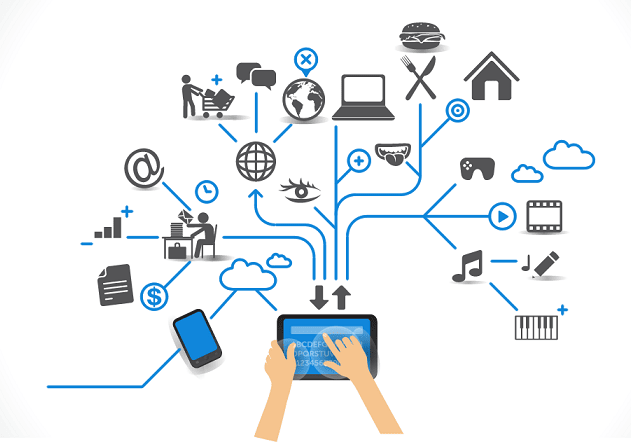
\includegraphics[scale=0.75]{Plataforma_internet.png}
	\caption[{Διαδίκτυο}]{Διαδίκτυο \textbf{Πηγή:} \cite{fig_Plataforma_internet}}
	\label{fig:Plataforma_internet}
\end{figure}

Το Διαδίκτυο μπορεί να χρησιμοποιηθεί για σχεδόν κάθε σκοπό που εξαρτάται από την πληροφορία, και όποιος έχει την δυνατότητα να συνδεθεί σε ένα από τα δίκτυα που το συνθέτουν, έχει πρόσβαση σε αυτό. Υποστηρίζει την ανθρώπινη επικοινωνία μέσω των κοινωνικών μέσων, του ηλεκτρονικού ταχυδρομείου (e-mail), των ``chat rooms'', και επιτρέπει στους ανθρώπους να συνεργάζονται είτε σύγχρονα, είτε ασύγχρονα σε πολλά διαφορετικά μέρη του κόσμου. Υποστηρίζει την πρόσβαση σε ψηφιακές πληροφορίες μέσω πολλών εφαρμογών, συμπεριλαμβανομένου του Παγκόσμιου Ιστού. Το Διαδίκτυο έχει διαδραματίσει σημαντικό ρόλο στην ανάπτυξη ενός μεγάλου και αυξανόμενου αριθμού ``ηλεκτρονικών επιχειρήσεων'' (συμπεριλαμβανομένων και των θυγατρικών των παραδοσιακών εταιρειών) που χρησιμοποιούν το Διαδίκτυο για το μεγαλύτερο μέρος των πωλήσεων και των υπηρεσιών τους.

\subsection{Παγκόσμιος Ιστός}
Αν και μερικές φορές χρησιμοποιούνται ως όμοιοι, οι όροι Διαδίκτυο και Παγκόσμιος Ιστός δεν έχουν την ίδια σημασία. Ο Παγκόσμιος Ιστός είναι μία από τις κύριες υπηρεσίες που παρέχονται μέσω του Διαδικτύου, ενώ ο όρος ``Διαδίκτυο'' αναφέρεται σε ολόκληρο το παγκόσμιο σύστημα επικοινωνίας, που περιλαμβάνει το υλικό και την υποδομή. Πιο επίσημα, ο Παγκόσμιος Ιστός μπορεί να οριστεί ως ένα σύστημα τεχνικοκοινωνικής αλληλεπίδρασης. Ένα σύστημα που βελτιώνει την ανθρώπινη διάνοια, την επικοινωνία και τη συνεργασία αναφέρεται ως τεχνοκοινωνικό σύστημα. Οι πληροφορίες που δημιουργούνται στον Παγκόσμιο Ιστό από τους χρήστες του μπορούν να αποθηκεύονται στο Διαδίκτυο. Υπάρχουν διάφοροι ιστότοποι στον Παγκόσμιο Ιστό, καθένας από τους οποίους έχει τη δική του διεύθυνση URL (Uniform Resource Locator). Η διεύθυνση URL έχει τη μορφή http://www.example.com. Το http συνιστά τη βάση δεδομένων επικοινωνίας για τον Παγκόσμιο Ιστό, το www πρόκειται για το World Wide Web, το οποίο είναι ένα πληροφοριακό σύστημα όπου τα έγγραφα και άλλοι δικτυακοί τόποι αναγνωρίζονται από τις διευθύνσεις URL τους, το example δηλώνει το όνομα του δικτυακού τόπου (domain name) και το com υποδεικνύει την περιοχή στην οποία ανήκει ο δικτυακός τόπος ή τον τύπο του δικτυακού τόπου \cite{aghaei2012evolution}.

\subsection{Εφαρμογή Ιστού}
Μια Εφαρμογή Web (Ιστού) συνιστά μια εφαρμογή που διανέμεται μέσω του Διαδικτύου με τη χρήση ενός προγράμματος περιήγησης και διατηρείται σε έναν απομακρυσμένο διακομιστή. Εξ ορισμού, οι υπηρεσίες διαδικτύου είναι Εφαρμογές Ιστού και πολλοί ιστότοποι -αν και όχι όλοι- περιέχουν τέτοιες εφαρμογές. Οι Εφαρμογές Ιστού μπορούν να δημιουργηθούν για ένα ευρύ φάσμα σκοπών και να χρησιμοποιηθούν από ανθρώπους ή οργανισμούς για πολλά διαφορετικά πράγματα. Το webmail, οι ηλεκτρονικές αριθμομηχανές και οι ιστότοποι ηλεκτρονικών αγορών είναι μερικά παραδείγματα συχνά χρησιμοποιούμενων Εφαρμογών Ιστού. Αν και η πλειονότητα των εφαρμογών ιστού είναι προσβάσιμες από οποιοδήποτε πρόγραμμα περιήγησης, ορισμένες απαιτούν συγκεκριμένο λογισμικό για την ορθή λειτουργία τους και τη βέλτιστη εμπειρία του χρήστη τους \cite{Web_Apps}.

\section{Τεχνικές Προγραμματισμού}

\subsection{Αντικειμενοστρεφής Προγραμματισμός}
Ο αντικειμενοστρεφής προγραμματισμός (Object Oriented Programming / OOP), αποτελεί πρότυπο στην ανάπτυξη εφαρμογών, σε οποιαδήποτε γλώσσα. Βασίζεται στις ιδέες των κλάσεων και των αντικειμένων. Χρησιμοποιείται για την οργάνωση του λογισμικού σε απλές, επαναχρησιμοποιήσιμες κλάσεις σχεδίων κώδικα, οι οποίες στη συνέχεια χρησιμοποιούνται για τη δημιουργία ξεχωριστών περιπτώσεων αντικειμένων. Οι γλώσσες αντικειμενοστρεφούς προγραμματισμού JavaScript, C++, Java, Python και PHP είναι μερικά μόνο παραδείγματα \cite{smith2011object}.

Μια κλάση είναι ένα γενικευμένο πρότυπο που μπορεί να χρησιμοποιηθεί για τη δημιουργία πιο εξειδικευμένων, συγκεκριμένων πραγμάτων. Ευρείες κατηγορίες με κοινές ιδιότητες αναπαρίστανται συχνά με τη χρήση κλάσεων. Αυτές οι κλάσεις καθορίζουν τα χαρακτηριστικά μιας περίπτωσης τύπου, όπως το χρώμα, αλλά όχι την τιμή αυτών των χαρακτηριστικών για ένα συγκεκριμένο αντικείμενο.

Οι κλάσεις μπορούν επίσης να περιλαμβάνουν μεθόδους, οι οποίες είναι ειδικές λειτουργίες προσβάσιμες μόνο από αντικείμενα αυτού του είδους. Αυτές οι συναρτήσεις, οι οποίες ορίζονται εντός της κλάσης, εκτελούν ορισμένες χρήσιμες ενέργειες για το συγκεκριμένο είδος αντικειμένου.

Η δημιουργία μοναδικών αντικειμένων ακολουθεί το σχέδιο που παρέχουν τα πρότυπα κλάσεων. Κάθε αντικείμενο μπορεί να έχει διαφορετική τιμή για κάθε μία από τις δηλωμένες ιδιότητες της κλάσης \cite{Doherty_2020}.

\subsection{Αρχιτεκτονική MVC}
Το MVC είναι ένα αρχιτεκτονικό πρότυπο, το οποίο υποδηλώνει ότι ελέγχει ολόκληρο το σχεδιασμό της εφαρμογής. Παρόλο που αναφέρεται συχνά ως πρότυπο σχεδίασης, αυτό μπορεί να είναι ανακριβές, διότι τα πρότυπα σχεδίασης χρησιμοποιούνται για την αντιμετώπιση ορισμένων τεχνικών ζητημάτων, αλλά τα πρότυπα αρχιτεκτονικής αντιμετωπίζουν αρχιτεκτονικά ζητήματα, έχοντας αντίκτυπο σε ολόκληρο τον σχεδιασμό του προγράμματος \cite{Svirca_2020}. Κατά την ανάπτυξη μιας εφαρμογής, είναι απαραίτητη η οργάνωση του κώδικα, έτσι ώστε η πρόσβαση στα κατάλληλα αρχεία και η συντήρηση τους να είναι εύκολη και διαισθητική. Η οργάνωση των αρχείων της εφαρμογής με τη χρήση του προτύπου Model, View, Controller (MVC) επιτυγχάνει τη διατήρηση των δεδομένων, της εμφάνισης και της ροής της εφαρμογής διακριτά \cite{CodeIgniter_mvc}.

Όπως φαίνεται και στο σχήμα \ref{fig:mvc-arch}, υπάρχουν τρία βασικά μέρη σε αυτό: τα \hyperref[thb:Models]{Models} για την επικοινωνία της εφαρμογής με τη βάση δεδομένων, τα \hyperref[thb:Views]{Views} για την απεικόνιση των πληροφοριών και οι \hyperref[thb:Controllers]{Controllers} για την υλοποίηση της επιχειρηματικής λογικής της εφαρμογής. Επίσης, ένα συμπληρωματικό βοηθητικό στοιχείο είναι τα \hyperref[thb:Entities]{Entities}, τα οποία προσφέρουν αντικειμενοστρέφεια στις γραμμές αποτελεσμάτων που επιστρέφονται από τη βάση δεδομένων μέσω των Models.

\begin{figure}[h]
	\centering
	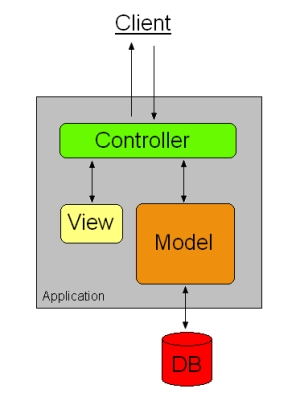
\includegraphics[scale=0.75]{MVC_Diagram_3.jpg}
	\caption[{Διάγραμμα Αρχιτεκτονικής MVC}]{Διάγραμμα Αρχιτεκτονικής MVC \textbf{Πηγή:} \cite{fig_MVC_Diagram_3}}
	\label{fig:mvc-arch}
\end{figure}

\subsubsection{Models} \label{thb:Models}
Τα μοντέλα διαχειρίζονται τα δεδομένα της εφαρμογής και βοηθούν στην επιβολή τυχόν ειδικών επιχειρησιακών κανόνων που μπορεί να χρειάζεται η εφαρμογή. Η δουλειά ενός μοντέλου είναι να διαχειρίζεται έναν συγκεκριμένο τύπο δεδομένων για την εφαρμογή. Αυτό μπορεί να είναι χρήστες, αναρτήσεις σε ιστολόγια, συναλλαγές κ.α. Σε αυτή την περίπτωση, η δουλειά του μοντέλου έχει δύο μέρη: να επιβάλλει επιχειρηματικούς κανόνες στα δεδομένα καθώς αυτά αντλούνται από τη βάση δεδομένων ή τοποθετούνται σε αυτήν και να χειρίζεται την πραγματική αποθήκευση και ανάκτηση των δεδομένων από τη βάση δεδομένων. Η επιβολή επιχειρηματικών κανόνων μπορεί να περιλαμβάνει την κανονικοποίηση των ακατέργαστων δεδομένων πριν από την αποθήκευση, ώστε να πληρούν τις απαραίτητες προδιαγραφές ασφαλείας, ή τη μορφοποίηση μιας στήλης με συγκεκριμένο τρόπο πριν από την παράδοσή της στον ελεγκτή. Διατηρώντας αυτές τις επιχειρηματικές απαιτήσεις στο μοντέλο, δεν επαναλαμβάνεται κώδικας σε πολλούς ελεγκτές, κατά την ανάκτηση δεδομένων από τη βάση ή πριν την αποθήκευσή τους σε αυτή.

\subsubsection{Views} \label{thb:Views}
Το στοιχείο προβολής χειρίζεται την αναπαράσταση δεδομένων. Στην πραγματικότητα, δημιουργεί τη διεπαφή χρήστη (UI) για τον χρήστη. Τα δεδομένα που συγκεντρώνει το συστατικό μοντέλο για τις προβολές λαμβάνονται μέσω του ελεγκτή και όχι απευθείας, επομένως η προβολή επικοινωνεί μόνο με τον ελεγκτή \cite{tutorials_2022}.

Οι προβολές είναι τα πιο απλογραμμένα αρχεία και συχνά είναι μόνο HTML με πολύ λίγη PHP. Η PHP θα πρέπει να διατηρείται όσο το δυνατόν πιο βασική, συνήθως εμφανίζει τα περιεχόμενα μιας μεταβλητής ή εκτελεί επαναλήψεις σε διάφορα στοιχεία για την εμφάνιση των πληροφοριών τους.

Τα δεδομένα για τις προβολές προέρχονται από τους ελεγκτές, οι οποίοι τα στέλνουν στις προβολές ως μεταβλητές που μπορούν να εμφανιστούν με απλές κλήσεις echo. Άλλες προβολές μπορούν να εμφωλευθούν μέσα σε μια προβολή, καθιστώντας απλή την εμφάνιση μιας συνεπούς κεφαλίδας ή υποσέλιδου σε κάθε σελίδα.

\subsubsection{Controllers} \label{thb:Controllers}
Οι ελεγκτές μπορούν να αναλάβουν δύο διαφορετικά καθήκοντα. Το πρώτο και πιο προφανές είναι ότι δέχονται την είσοδο του χρήστη και στη συνέχεια αποφασίζουν τι να κάνουν με αυτήν. Αυτό συχνά συνεπάγεται την παράδοση των δεδομένων σε ένα μοντέλο για τη διατήρησή τους ή την αίτηση δεδομένων από το μοντέλο για να παρουσιαστούν από την προβολή. Αυτό περιλαμβάνει επίσης τη φόρτωση επιπλέον βοηθητικών κλάσεων, αν είναι απαραίτητο, για την εκπλήρωση εξειδικευμένων δραστηριοτήτων που δεν καλύπτονται από το μοντέλο.

Ο ελεγκτής είναι επίσης υπεύθυνος για το χειρισμό όλων όσων σχετίζονται με τα αιτήματα HTTP, όπως η ανακατεύθυνση, ο έλεγχος ταυτότητας, η ασφάλεια ιστού, η κωδικοποίηση κ.ο.κ. Συνοπτικά, ο ελεγκτής διασφαλίζει ότι επιτρέπεται η πρόσβαση και ότι τα δεδομένα που χρειάζονται παρέχονται σε μορφή που μπορούν να χρησιμοποιήσουν.

Ως το συστατικό που παρέχει τη σύνδεση μεταξύ των προβολών και του μοντέλου, ο ελεγκτής αναφέρεται ως ο ``κύριος ρόλος'', δεδομένου ότι λειτουργεί ως ενδιάμεσος. Ο ελεγκτής χρειάζεται μόνο να δίνει οδηγίες στο μοντέλο - δεν χρειάζεται να ανησυχεί για το χειρισμό της λογικής των δεδομένων. Αφού επεξεργαστεί τα δεδομένα που έχει λάβει από το μοντέλο, τα στέλνει στην προβολή και δίνει οδηγίες στον χρήστη για τον τρόπο απεικόνισής τους. Οι προβολές και τα μοντέλα δεν μπορούν να συνομιλούν άμεσα, παρά μόνο με την διαμεσολάβηση κάποιου ελεγκτή.

\subsubsection{Entities} \label{thb:Entities}
Οι κλάσεις οντοτήτων υποστηρίζονται ως πολίτες πρώτης κατηγορίας στο επίπεδο της βάσης δεδομένων, διατηρώντας παράλληλα την χρήση τους εντελώς προαιρετική.

Στον πυρήνα της, μια κλάση οντότητας είναι απλά μια κλάση που αναπαριστά μια μεμονωμένη γραμμή βάσης δεδομένων. Έχει ιδιότητες κλάσης για να αναπαριστά τις στήλες της βάσης δεδομένων και παρέχει οποιεσδήποτε πρόσθετες μεθόδους για την υλοποίηση της επιχειρηματικής λογικής για αυτή τη γραμμή. Το βασικό χαρακτηριστικό, όμως, είναι ότι δεν γνωρίζει τίποτα για το πώς να διατηρείται η ίδια. Αυτό είναι ευθύνη του μοντέλου ή της κλάσης αποθετηρίου. Με αυτόν τον τρόπο, αν αλλάξει κάτι σχετικά με τον τρόπο που πρέπει να αποθηκεύσετε το αντικείμενο, δεν χρειάζεται να αλλάξετε τον τρόπο με τον οποίο χρησιμοποιείται αυτό το αντικείμενο σε όλη την εφαρμογή.

\subsection{RESTful API}
Η μεταφορά κατάστασης παρουσίασης (REpresentational State Transfer), κοινώς γνωστή ως REST, είναι ένας αρχιτεκτονικός σχεδιασμός για κατανεμημένα συστήματα υπερμέσων. Παρουσιάστηκε για πρώτη φορά στη διάσημη διατριβή του Roy Fielding από το 2000.
Οι κατευθυντήριες έννοιες και οι περιορισμοί του REST είναι παρόμοιοι με εκείνους άλλων αρχιτεκτονικών στυλ. Εάν μια διεπαφή υπηρεσίας θέλει να αναφέρεται ως RESTful, πρέπει να τηρεί αυτά τα πρότυπα \cite{Gupta_2020}.

\begin{figure}[ht]
	\centering
	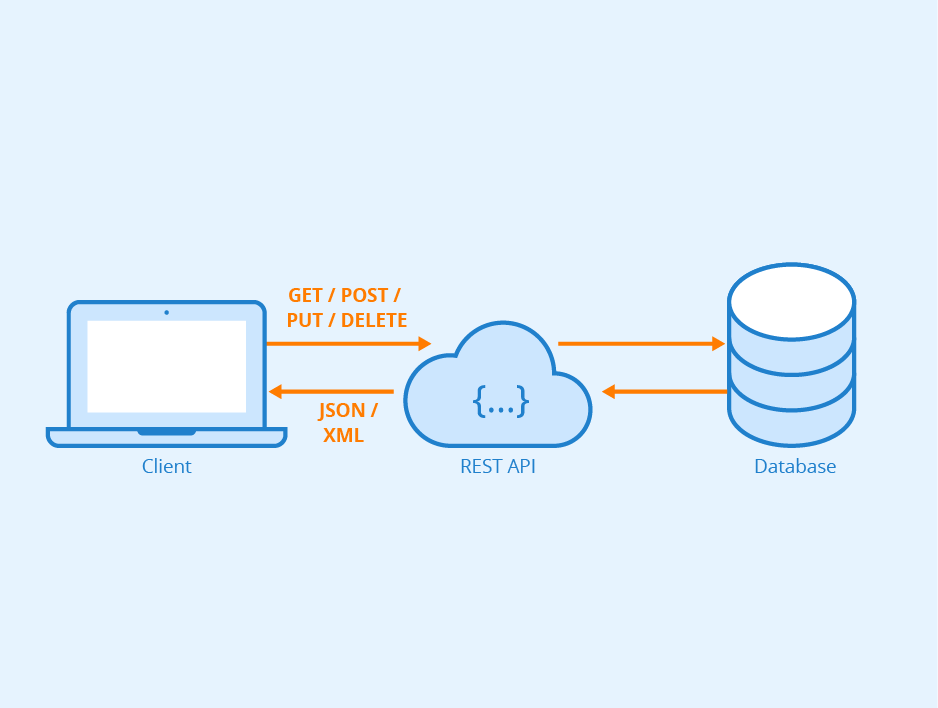
\includegraphics[scale=0.4]{Rest-API.png}
	\caption[{REST API}]{REST API \textbf{Πηγή:} \parencite{fig_Rest_API}}
	\label{fig:rest_api}
\end{figure}

Ένα σύνολο ορισμών και πρωτοκόλλων, γνωστό ως API, χρησιμοποιείται για τη δημιουργία και την ενσωμάτωση λογισμικού εφαρμογών. Μερικές φορές αναφέρεται ως σύμβαση μεταξύ ενός παρόχου πληροφοριών και ενός χρήστη αυτών των πληροφοριών, η οποία περιγράφει το περιεχόμενο που ο καταναλωτής (η κλήση) και ο παραγωγός υποχρεούνται να παραδώσουν (η απάντηση). Το API περιγράφει τον τρόπο με τον οποίο ένας προγραμματιστής θα πρέπει να σχεδιάσει ένα πρόγραμμα που ζητά υπηρεσίες από ένα λειτουργικό σύστημα ή μια άλλη εφαρμογή. 

Ένα API μπορεί να θεωρηθεί ως μεσάζων μεταξύ των χρηστών ή των πελατών και των πόρων ή των επιγραμμικών υπηρεσιών στις οποίες προσπαθούν να έχουν πρόσβαση. Επιπλέον, παρέχει σε μια εταιρεία έναν μηχανισμό για την κοινή χρήση περιουσιακών στοιχείων και δεδομένων, διατηρώντας παράλληλα την αυθεντικοποίηση, τον έλεγχο και την ασφάλεια - αποφασίζοντας ποιος έχει πρόσβαση σε τι \cite{RedHat_2020}. 

Ένα RESTful API βασίζεται στην αναπαραστατική μεταφορά κατάστασης (REST), ένα αρχιτεκτονικό στυλ και μια προσέγγιση επικοινωνίας που χρησιμοποιείται συχνά στην κατασκευή υπηρεσιών ιστού. Είναι επίσης γνωστό ως RESTful υπηρεσία ιστού ή REST API.

Γενικά, η τεχνολογία REST προτιμάται έναντι άλλων, συγκρίσιμων τεχνολογιών. Αυτό συμβαίνει συχνά, καθώς η REST απαιτεί μικρότερο εύρος ζώνης και, ως εκ τούτου, είναι πιο κατάλληλη για την αποτελεσματική χρήση του διαδικτύου. Επιπλέον, γλώσσες υπολογιστών όπως η PHP, η JavaScript ή η Python μπορούν να χρησιμοποιηθούν για τη δημιουργία RESTful API \cite{Gillis_2020}.

\section{Γλώσσες Προγραμματισμού Ιστού}

\subsection{HTML}
Η HTML (Hyper Text Markup Language - Γλώσσα Σήμανσης Υπερκειμένου) αποτελεί την βασική γλώσσα για την κατασκευή ενός ιστοχώρου. Δεν θεωρείται γλώσσα προγραμματισμού, αλλά αποτελεί μία περιγραφική γλώσσα (markup language) η οποία περιέχει οδηγίες προς τους web browsers. Οι web browsers αφού διαβάσουν τις οδηγίες αυτές, τις μεταφράζουν στις κατάλληλες εντολές για να δημιουργηθεί το οπτικό περιεχόμενο που θα παρουσιαστεί στον χρήστη. Η παραπάνω διαδικασία επιτυγχάνεται με την βοήθεια των HTML elements, τα οποία οριοθετούνται από ετικέτες (tags). Οι ετικέτες είναι γράμματα ή λέξεις, τα οποία περικλείουν γωνιώδεις αγκύλες και υπάρχουν ανά ζεύγη. Χωρίζονται σε tags έναρξης, τα οποία σηματοδοτούν την έναρξη μιας εντολής, και σε tags λήξης, τα οποία σηματοδοτούν την λήξη της εντολής, με μερικές εξαιρέσεις. Οι ετικέτες λήξης διαχωρίζονται από τις ετικέτες έναρξης με μία πλάγια γραμμή '/'. Ένα βασικό παράδειγμα ετικέτας είναι το: <html>...</html>, ανάμεσα στις ετικέτες περικλείεται κείμενο ή ακόμη και άλλες εσωτερικές ετικέτες (εμφωλευμένα tags). Ορισμένες βασικές ετικέτες παρατίθενται στον πίνακα \ref{tbl:html_basic_elements}.

\begin{longtable}{|p{0.2\linewidth}|p{0.7\linewidth}|} 
	\caption{Βασικά στοιχεία HTML} \label{tbl:html_basic_elements} \\
	\hline
	\endfirsthead
	\caption[{}]{Βασικά στοιχεία HTML (συνέχεια)} \\ 
	\endhead \endfoot 
	\textless{}html\textgreater{}...\textless{}/html\textgreater{} & Η αρχή και το τέλος του HTML αρχείου \\ \hline
	\textless{}!DOCTYPE\textgreater{} & Η οδηγία που καθορίζει την έκδοση της HTML που χρησιμοποιείται \\ \hline
	\textless{}head\textgreater{}...\textless{}/head\textgreater{} & Οι σχετικές πληροφορίες με το έγγραφο (όπως η γλώσσα, η κωδικοποίηση και τα μεταδεδομένα) \\ \hline
	\textless{}title\textgreater{}...\textless{}/title\textgreater{} & Ο τίτλος του αρχείου \\ \hline
	\textless{}body\textgreater{}...\textless{}/body\textgreater{} & Τα οπτικά στοιχεία του αρχείου \\ \hline
	\textless{}div\textgreater{}...\textless{}/div\textgreater{} & Ομαδοποίηση στοιχείων εντός ετικέτας \\ \hline
	\textless{}input\textgreater{}...\textless{}/input\textgreater{} & Ορισμός πεδίου εισαγωγής \\ \hline
	\textless{}!--...--\textgreater{} & Ορισμός σχολίων \\ \hline
	\textless{}form\textgreater{}...\textless{}/form\textgreater{} & Ορισμός φόρμας \\ \hline
	\textless{}button\textgreater{}...\textless{}/button\textgreater{} & Ορισμός κουμπιού \\ \hline
	\textless{}a\textgreater{}...\textless{}/a\textgreater{} & Ορισμός υπερσυνδέσμου \\ \hline
\end{longtable}

\subsection{CSS}
Η CSS αποτελεί μία γλώσσα επικαλυπτόμενων στυλ μορφοποίησης (Cascading Style Sheets) και όπως η HTML δεν θεωρείται καθαρή γλώσσα προγραμματισμού. Συντελεί στον διαχωρισμό των εντολών εμφάνισης από τις εντολές του περιεχομένου της ιστοσελίδας. Χρησιμοποιείται για τη μορφοποίηση οποιασδήποτε ετικέτας HTLM και τη δημιουργία ενός αποτελέσματος πιο όμορφου οπτικά για τον χρήστη. Η σύνταξη μιας εντολής στην CSS αποτελείται από τρία κύρια στοιχεία: το στοιχείο που θα τροποποιηθεί, τις ιδιότητες του στοιχείου που θα επηρεαστούν και η νέα τιμή των ιδιοτήτων. Στον πίνακα \ref{tbl:css_basic_elements} αναφέρεται ένα παράδειγμα του τρόπου σύνταξης μιας εντολής στην γλώσσα CSS.

\begin{table}[h]
	\caption{Στοιχεία εντολής CSS}
	\label{tbl:css_basic_elements}
	\centering
	\begin{tabular}{|l|}
		\hline
		\begin{tabular}[c]{@{}l@{}}
			p \{ \\ \quad 
			font-family: Calibri; \\ \quad 
			color: \#1B1811; \\ \quad 
			text-align: left; \\ \}
		\end{tabular} \\ \hline
	\end{tabular}
\end{table}

Όπως φαίνεται στον πίνακα \ref{tbl:css_basic_elements}, το στοιχείο p αποτελεί την ετικέτα της παραγράφου στην HTML και ονομάζεται επιλογέας (css selector). Τα font-family, color και text-align είναι οι ιδιότητες της εντολής CSS και δείχνουν τα στοιχεία του επιλογέα τα οποία θα τροποποιηθούν. Ο διαχωρισμός των ιδιοτήτων από τις νέες τιμές που θα λάβουν σηματοδοτείται με την άνω και κάτω τελεία (:), στης οποίας το αριστερό μέρος βρίσκονται οι ιδιότητες και στο δεξί οι νέες τιμές τους.

\subsection{JavaScript \& Ajax}
Η JavaScript είναι μια γλώσσα προγραμματισμού σεναρίου (scripting language), η οποία εκτελείται από τους περιηγητές ιστών (web browsers) χρησιμοποιώντας έναν σχετικό διερμηνευτή (Interpreter). Στόχο της αποτελεί η βελτίωση της εμπειρίας χρήσης. Με την JavaScript υπάρχει η δυνατότητα προσθήκης ή αφαίρεσης HTML στοιχείων και CSS κανόνων καθώς και η τροποποίηση ιδιοτήτων HTLM στοιχείων με την μεταβολή στις τιμές τους. Αν και η JavaScript αποτελεί μια γλώσσα προγραμματισμού με το Client-Side χαρακτηριστικό, τον τελευταίο καιρό γίνεται χρήση της και από την πλευρά των υπολογιστών εξυπηρετητών.

Η Ajax (Asynchronous JavaScript and XML) αποτελείται από τον συνδυασμό των τεχνολογιών JavaScript και XML. Είναι μία τεχνολογία, η οποία προσδίδει διαδραστικές δυνατότητες σε μία ιστοσελίδα. Μέσω της Ajax γίνεται εφικτή η ανανέωση μέρους της ιστοσελίδας (στο παρασκήνιο θα γίνει επικοινωνία της τεχνολογίας με τον server, ο οποίος θα λάβει τα δεδομένα που ζητήθηκαν και με τη σειρά του θα τα εμφανίσει στον χρήστη), χωρίς να χρειαστεί να γίνει ανανέωση (refresh) ολόκληρης της ιστοσελίδας.

\subsection{PHP}
Η PHP ορίζεται ως μία αντικειμενοστρεφής γλώσσα προγραμματισμού γενικής χρήσης (παλαιότερα αποτελούσε γλώσσα προγραμματισμού σεναρίου), η οποία χρησιμοποιείται κυρίως για την ανάπτυξη διαδικτυακών εφαρμογών (web apps), δηλαδή αποτελεί την κατάλληλη γλώσσα για την δημιουργία ιστοχώρων με δυναμικό περιεχόμενο. Διατίθεται σε δύο μορφές, σε μορφή πηγαίου κώδικα και σε δυαδική μορφή και οι δύο αυτές μορφές έχουν ελεύθερη πρόσβαση. Η PHP χρησιμοποιείται για τον χειρισμό λειτουργιών και εργασιών τις οποίες θα υλοποιήσει και όχι για την οπτική διαμόρφωση μίας ιστοσελίδας.

Επομένως, ο χρήστης λαμβάνει τα αποτελέσματα του σεναρίου (στον browser ως απλές σελίδες HTLM) και όχι τον κώδικα, ο οποίος εκτελείται στον server με τη χρήση του αντίστοιχου διερμηνευτή (interpreter) της κάθε γλώσσας. Ο διερμηνευτής, αφού διαβάσει τον κώδικα, εκτελεί τις δηλώσεις της γλώσσας ανά βήμα και τις μετατρέπει σε εκτελέσιμο κώδικα για το υπολογιστικό σύστημα.

Αναλυτικότερα, η PHP έχει την ικανότητα να δημιουργήσει, γράψει, διαβάσει, ανοίξει, κλείσει και διαγράψει αρχεία στη Βάση Δεδομένων. Υποστηρίζει ένα ευρύ φάσμα Βάσεων Δεδομένων, καθώς επίσης είναι δωρεάν και αρκετά εύκολη στην εκμάθηση, ενώ ταυτόχρονα είναι συμβατή και μπορεί να τρέξει σε οποιαδήποτε πλατφόρμα, όπως για παράδειγμα Windows, Mac OS, Linux, Unix κ.α. Ένα αρχείο PHP (έγγραφο κειμένου αποθηκευμένο με την κατάληξη .php) είναι δυνατό να περιέχει εκτός από τον κώδικα PHP και κώδικα HTLM, CSS και JavaScript.

Ορισμένες βασικές συναρτήσεις της PHP παρατίθενται στον πίνακα \ref{tbl:php_basic_functions}.

\begin{longtable}{|p{0.2\linewidth}|p{0.7\linewidth}|} 
	\caption{Βασικές συναρτήσεις της PHP} \label{tbl:php_basic_functions} \\
	\hline
	\endfirsthead
	\caption[{}]{Βασικές συναρτήσεις της PHP (συνέχεια)} \\ 
	\endhead \endfoot 
	htmlspecialchars() & Μετατροπή ειδικών χαρακτήρων σε οντότητες HTML \\ \hline
	explode() & Μετατροπή μιας συμβολοσειράς σε πίνακα με χρήση ενός διαχωριστικού χαρακτήρα \\ \hline
	rand() & Επιστροφή ενός τυχαίου αριθμού \\ \hline
	str\_replace() & Εύρεση και αντικατάσταση ενός μοτίβου σε μια συμβολοσειρά \\ \hline
	date() & Επιστροφή μιας μορφοποιημένης ημερομηνίας \\ \hline
	strlen() & Επιστροφή του μήκους μιας συμβολοσειράς \\ \hline
	count() & Επιστροφή του αριθμού των στοιχείων ενός πίνακα \\ \hline
	array\_unique() & Απαλοιφή διπλότυπων στοιχείων ενός πίνακα \\ \hline
	print\_r() & Εκτύπωση μεταβλητής \\ \hline
	echo & Εκτύπωση μίας ή περισσότερων συμβολοσειρών \\ \hline
\end{longtable}

\subsection{SQL}
Η τυποποιημένη γλώσσα προγραμματισμού Structured Query Language (SQL) \cite{Loshin_2022}, χρησιμοποιείται για τη διαχείριση σχεσιακών βάσεων δεδομένων και την εκτέλεση διαφόρων πράξεων στα δεδομένα που περιέχουν. Από την ίδρυσή της τη δεκαετία του 1970, η SQL χρησιμοποιείται ευρέως από διαχειριστές βάσεων δεδομένων καθώς και από προγραμματιστές που δημιουργούν σενάρια για την ολοκλήρωση δεδομένων και από αναλυτές δεδομένων που κατασκευάζουν και εκτελούν αναλυτικά ερωτήματα.

Με τη βοήθεια της ευέλικτης γλώσσας SQL, οι χρήστες μπορούν να λαμβάνουν, να αποθηκεύουν, να επεξεργάζονται και να διαγράφουν δεδομένα, καθώς και να δημιουργούν, να τροποποιούν και να αφαιρούν αντικείμενα βάσεων δεδομένων (όπως πίνακες, στήλες, διαδικασίες και χρήστες), καθώς και να δίνουν και να ανακαλούν προνόμια χρηστών και να ομαδοποιούν δηλώσεις σε συναλλαγές. Μια δήλωση που ζητά δεδομένα από τη βάση δεδομένων αναφέρεται ως ερώτημα και μια εντολή SQL είναι γνωστή ως δήλωση. Στις εντολές SQL περιλαμβάνονται προγνωστικά (όπως LIKE, BETWEEN, EXISTS), τελεστές (όπως AND, OR, NOT), ποσοδείκτες (όπως ANY, ALL, UNION), συναρτήσεις (όπως COUNT, SUM, AVG) και προτάσεις (όπως SELECT, FROM, WHERE). Όταν δεν είναι σημαντικό να γίνει διάκριση μεταξύ, για παράδειγμα, των ρητρών και των κατηγορημάτων, αναφερόμαστε σε αυτά ως έννοιες συλλογικά.

Η γλώσσα χειρισμού δεδομένων (DML, π.χ. SELECT, INSERT, UPDATE, DELETE) και η γλώσσα ορισμού δεδομένων (DDL, π.χ. CREATE, ALTER, DROP) είναι οι δύο υπογλώσσες της SQL που χρησιμοποιούνται συχνότερα \cite{taipalus2020sql}.
 
Τα δεδομένα αποθηκεύονται, ανακτώνται και αναλύονται με τη χρήση λογισμικού που ονομάζεται σύστημα διαχείρισης βάσεων δεδομένων (DBMS). Οι χρήστες μπορούν να δημιουργούν, να διαβάζουν, να ενημερώνουν και να διαγράφουν δεδομένα σε βάσεις δεδομένων χρησιμοποιώντας ένα DBMS, το οποίο λειτουργεί ως διεπαφή μεταξύ αυτών και των βάσεων δεδομένων. Η ασφάλεια των δεδομένων, η ακεραιότητα των δεδομένων, η ταυτόχρονη χρήση και οι τυποποιημένες πρακτικές διαχείρισης δεδομένων βοηθούνται από αυτό.

Τα μοντέλα δεδομένων, οι κατανομές βάσεων δεδομένων, ο αριθμός των χρηστών και άλλοι παράγοντες μπορούν να χρησιμοποιηθούν για την κατηγοριοποίηση των συστημάτων διαχείρισης βάσεων δεδομένων. Οι σχεσιακές, κατανεμημένες, ιεραρχικές, αντικειμενοστραφείς και δικτυακές μορφές λογισμικού DBMS είναι οι πιο δημοφιλείς \cite{DBMS}.

Στα συστήματα διαχείρισης σχεσιακών βάσεων δεδομένων (RDBMS), η SQL χρησιμοποιείται για τις ακόλουθες εργασίες: αλλαγή των δομών των πινάκων και των δεικτών της βάσης δεδομένων, προσθήκη, ενημέρωση και διαγραφή γραμμών δεδομένων και ανάκτηση υποσυνόλων πληροφοριών. Οι πληροφορίες αυτές μπορούν να χρησιμοποιηθούν για την επεξεργασία συναλλαγών, εφαρμογές ανάλυσης και άλλες εφαρμογές που απαιτούν αλληλεπίδραση με μια σχεσιακή βάση δεδομένων.

\section{Πλαίσια και Βιβλιοθήκες Προγραμματισμού Ιστού}

\subsection{Bootstrap}
Μια βιβλιοθήκη HTML, CSS και JS με έμφαση στη βελτιστοποίηση της διαδικασίας ανάπτυξης ιστοσελίδων ονομάζεται Bootstrap (σε αντίθεση με τις εφαρμογές ιστού). Το Bootstrap είναι ένα δωρεάν και ανοικτού κώδικα πλαίσιο CSS που δημιουργήθηκε αρχικά από το Twitter και σήμερα αναπτύσσεται από την ομάδα του Bootstrap στο Github. Σκοπός του είναι να αποτελέσει τα θεμέλια για την ανάπτυξη front-end ιστοσελίδων που δίνουν προτεραιότητα στη καλή εμπειρία χρήσης από κινητές συσκευές. Προσφέρει πρότυπα σχεδίασης HTML, CSS και (προαιρετικά) JavaScript για τυπογραφία, φόρμες, κουμπιά, πλοήγηση και άλλα στοιχεία διεπαφής \cite{Bootstrap}. 

Ο κύριος στόχος της προσθήκης του σε ένα έργο ιστού είναι η εφαρμογή των επιλογών χρώματος, μεγέθους, γραμματοσειράς και διάταξης του Bootstrap σε αυτό το έργο. Ως εκ τούτου, ο κύριος καθοριστικός παράγοντας είναι το κατά πόσον αυτές οι επιλογές αρέσουν στους υπεύθυνους προγραμματιστές. Όλα τα στοιχεία HTML έχουν βασικές δηλώσεις στυλ μόλις το Bootstrap εισαχθεί σε ένα έργο. 

Ως αποτέλεσμα, τα κείμενα, οι πίνακες και τα στοιχεία φόρμας εμφανίζονται ομοιόμορφα σε όλα τα προγράμματα περιήγησης ιστού. Προκειμένου να εξατομικεύσουν περαιτέρω την εμφάνιση του περιεχομένου τους, οι προγραμματιστές μπορούν να κάνουν χρήση των κλάσεων CSS που ορίζονται στο Bootstrap. Για παράδειγμα, το Bootstrap προσφέρει ενσωματωμένη υποστήριξη για ανοιχτόχρωμους και σκούρους πίνακες, επικεφαλίδες σελίδων, μεγαλύτερα pull quotes και κείμενο με υπογράμμιση \cite{bootstrap_2}.

Επιπλέον, το Bootstrap περιλαμβάνει μια σειρά από στοιχεία JavaScript που μπορούν να χρησιμοποιηθούν ανεξάρτητα από άλλα πλαίσια, όπως το jQuery. Προσφέρουν επιπλέον στοιχεία UI, όπως πλαίσια διαλόγου, tooltips, μπάρες προόδου, drop-down μενού και καρουσέλ \cite{gaikwad2019review}. Κάθε στοιχείο Bootstrap αποτελείται από ένα πλαίσιο HTML, δηλώσεις CSS και περιστασιακά από συμπληρωματικό κώδικα JavaScript. Ταυτόχρονα, αυξάνουν τη λειτουργικότητα μερικών ήδη υπαρχόντων στοιχείων διεπαφής, όπως η λειτουργία αυτόματης συμπλήρωσης για τα πεδία εισαγωγής.

\subsection{CodeIgniter}
Το CodeIgniter είναι ένα πλαίσιο ανάπτυξης εφαρμογών MVC, διαθέσιμο για προγραμματιστές ιστοσελίδων PHP. Προσφέροντας μια ολοκληρωμένη συλλογή βιβλιοθηκών για συχνά εκτελούμενες λειτουργίες, καθώς και μια φιλική προς το χρήστη διεπαφή και μια λογική δομή πρόσβασης, στοχεύει να κάνει τη δημιουργία έργων σημαντικά ταχύτερη από τη συγγραφή κώδικα από το μηδέν. Το CodeIgniter προσπαθεί να γράφει όσο το δυνατόν λιγότερο κώδικα για την ολοκλήρωση μιας εργασίας \cite{Jackson_2020}.

Πρόκειται για ένα πλαίσιο με αμελητέες απαιτήσεις διαμόρφωσης. Προσφέρει εξαιρετικές επιδόσεις, διαθέτει λεπτομερή, σαφή τεκμηρίωση και δεν απαιτεί τη χρήση της γραμμής εντολών ή την τήρηση αυστηρών οδηγιών κωδικοποίησης. Αποφεύγει την πολυπλοκότητα και ευνοεί τις απλές διορθώσεις \cite{CodeIgniter_intro}.

\subsection{Swagger - OpenAPI}
Το Swagger είναι μια συλλογή οδηγιών, απαιτήσεων και πόρων ανοικτού κώδικα για τη δημιουργία και τον ορισμό RESTful APIs, τα οποία υλοποιούν τις προδιαγραφές του OpenAPI. Το έργο ξεκίνησε το 2011 από τον Tony Tam, ο οποίος εργαζόταν στη δημιουργία εργαλείων για τον ιστότοπο λεξικού Wordnik και πλέον συντηρείται από την SmartBear Software. Οι προγραμματιστές μπορούν να γράφουν διαδραστική, αναγνώσιμη από μηχανήματα και ανθρώπους τεκμηρίωση API χρησιμοποιώντας το πλαίσιο Swagger \cite{Swagger_2022}.

Πληροφορίες όπως υποστηριζόμενες λειτουργίες, παράμετροι και έξοδοι, ανάγκες εξουσιοδότησης, προσβάσιμα τελικά σημεία και απαιτούμενη αδειοδότηση περιλαμβάνονται συχνά στις προδιαγραφές API. Ζητώντας από το API να παραδώσει ένα αρχείο τεκμηρίωσης από τις επισημάνσεις του, το Swagger μπορεί να παράγει αυτόματα αυτές τις πληροφορίες από τον πηγαίο κώδικα.

Οι χρήστες μπορούν να δημιουργούν, να τεκμηριώνουν, να δοκιμάζουν και να καταναλώνουν RESTful υπηρεσίες ιστού με τη βοήθεια του Swagger. Εφαρμόζεται τόσο σε μεθοδολογίες ανάπτυξης API από πάνω προς τα κάτω όσο και από κάτω προς τα πάνω. Το Swagger μπορεί να χρησιμοποιηθεί για τη δημιουργία ενός API στην προσέγγιση top-down ή ``design-first'', πριν αναπτυχθεί οποιοσδήποτε κώδικας. Η τεκμηρίωση παράγεται από το Swagger χρησιμοποιώντας τον κώδικα που δημιουργείται για ένα API στην προσέγγιση ``από κάτω προς τα πάνω'' ή ``code-first'' \cite{Swagger_2019}.

\filbreak
\section{Τεχνολογίες Ανάπτυξης Λογισμικού}

\subsection{Jetbrains PhpStorm}
Κατασκευασμένο από την τσεχική εταιρεία JetBrains, το PhpStorm είναι ένα ιδιόκτητο, διαπλατφορμικό IDE (ολοκληρωμένο περιβάλλον ανάπτυξης) για PHP \cite{grigorev2014string}. Με on-the-fly ανάλυση κώδικα, πρόληψη σφαλμάτων και αυτοματοποιημένες αναδιαμορφώσεις για κώδικα PHP και JavaScript, το PhpStorm προσφέρει έναν επεξεργαστή για PHP, HTML και JavaScript. Η PHP υποστηρίζεται από τη συμπλήρωση κώδικα του PhpStorm, η οποία υποστηρίζει επίσης namespaces, closures, traits, generators, coroutines, τη λέξη-κλειδί finally, λίστες σε foreach και σύνταξη σύντομων πινάκων. Περιλαμβάνεται ένας πλήρης επεξεργαστής SQL με επεξεργάσιμα αποτελέσματα ερωτημάτων.

Το PhpStorm είναι γραμμένο σε Java. Εγκαθιστώντας plugins που έχουν κατασκευαστεί για το PhpStorm ή δημιουργώντας τα δικά τους, οι χρήστες μπορούν να επεκτείνουν τη λειτουργικότητα του IDE. Επιπλέον, το λογισμικό αλληλεπιδρά με εξωτερικούς πόρους όπως το XDebug. Το PhpStorm περιέχει όλες τις δυνατότητες που υπάρχουν στο WebStorm. Τα πρόσθετα JavaScript είναι ήδη προεγκατεστημένα στο WebStorm \cite{PhpStorm_JetBrains}.

\subsection{Git - GitHub}
\subsubsection{Git}
Το Global Information Tracker (Git) είναι ένα σύστημα ελέγχου εκδόσεων (VCS) διαθέσιμο σε όλες τις κύριες πλατφόρμες ανάπτυξης μέσω μιας άδειας χρήσης ελεύθερου λογισμικού \cite{spinellis2012git}. Κύριο χαρακτηριστικό του git είναι η διευκόλυνση της κατανεμημένης ανάπτυξης μέσω πολλαπλών προγραμματιστών σε πολλαπλές τοποθεσίες, γεγονός που οδηγεί στην κλιμάκωση του χειρισμού ακόμη και χιλιάδων προγραμματιστών που εργάζονται στα ίδια ή διαφορετικά μέρη ενός έργου. Άλλα χαρακτηριστικά του αποτελούν η γρήγορη και αποδοτική συγχώνευση με τη χρήση τεχνικών ``delta'' και συμπίεσης, η διατήρηση της ακεραιότητας των δεδομένων με την κρυπτογραφική συνάρτηση κατακερματισμού (SHA1) και η επιβολή της λογοδοσίας. Επίσης, υποστηρίζει και ενθαρρύνει τη διακλαδισμένη και σε άλλες περιπτώσεις τη συγχωνευμένη ανάπτυξη. Μία ακόμη ιδιότητα του git είναι πως διαθέτει πλήρη αποθετήρια. Ένα αποθετήριο αποτελείται από πολλούς φακέλους και αρχεία τα οποία είναι προσβάσιμα από οποιονδήποτε έχει πρόσβαση στο ιδιωτικό αποθετήριο \cite{loeliger2012version}. 

Το Git διαθέτει έναν αριθμό από Graphical User Interfaces (GUI) πελάτες και ένας από αυτούς είναι το GitKraken \cite{gitkrakenwhatisit}, το οποίο αποτελεί ένα γραφικό περιβάλλον διαχείρισης git αποθετηρίων. Χρησιμοποιείται για την εύκολη και αποτελεσματική διαχείριση, την δημιουργία, αλλά και την συγχώνευση των διακλαδώσεων. Διαθέτει την δυνατότητα να ενσωματώνεται με τον λογαριασμό GitHub ή Bitbucket ενός χρήστη, καθώς επίσης μπορεί να προσαρμοστεί εύκολα στον χώρο εργασίας του χρήστη.

\subsubsection{GitHub}
Το GitHub είναι μία διαδικτυακή πλατφόρμα συνεργατικής φιλοξενίας κώδικα ανάπτυξης λογισμικού, που βασίζεται στο σύστημα ελέγχου εκδόσεων git. Μέσω του GitHub, οι προγραμματιστές έχουν την δυνατότητα να αντιγράψουν ένα αποθετήριο στον λογαριασμό τους (fork) και αφού πραγματοποιήσουν τις αλλαγές τους, τους δίνεται η δυνατότητα να προτείνουν  να ενσωματωθούν στο αρχικό αποθετήριο από τους συντηρητές του (pull request και merge). Οι προγραμματιστές μπορούν επίσης να ακολουθήσουν άλλους χρήστες, σχηματίζοντας έτσι ένα κύκλωμα ανταλλαγής πληροφοριών, όπου κάθε προγραμματιστής ενημερώνεται για εξελίξεις σχετικές με τα ενδιαφέροντα του \cite{kalliamvakou2014promises}. Εκτός από τις λειτουργίες του Git, το GitHub προσφέρει και μερικά επιπρόσθετα χαρακτηριστικά. Βοηθά στη διαχείριση της πρόσβασης και της συνεργασίας για έργα, παρέχοντας χαρακτηριστικά όπως είναι η παρακολούθηση σφαλμάτων, η διαχείριση των διαφόρων εργασιών και τα αιτήματα χαρακτηριστικών.

\section{Σύνοψη Κεφαλαίου 2}
Στο δεύτερο κεφάλαιο εξετάστηκαν οι μέθοδοι και οι γλώσσες προγραμματισμού που εφαρμόστηκαν για την επεξεργασία και την ανάπτυξη της διαδικτυακής εφαρμογής. Εκτός από τα εργαλεία προγραμματισμού, η διατριβή περιλαμβάνει επίσης μια λεπτομερή περιγραφή των εργαλείων λογισμικού που χρησιμοποιήθηκαν για την οργάνωση και την κατασκευή του πληροφοριακού συστήματος. 

Η κατασκευή της βάσης δεδομένων και η δομή και οργάνωση του συστήματος καλύπτονται στο επόμενο κεφάλαιο.
